\documentclass{standalone}
\usepackage{tikz}
\usepackage{ctex,siunitx}
\setCJKmainfont{Noto Serif CJK SC}
\usepackage{tkz-euclide}
\usepackage{amsmath}
\usetikzlibrary{patterns, calc}
\usetikzlibrary {decorations.pathmorphing, decorations.pathreplacing, decorations.shapes,}
\begin{document}
\small
\begin{tikzpicture}[>=latex,scale=1]
  \begin{scope}
  \draw [semithick](-.25, -.4) rectangle (.25, .4);
  \draw [thick,<->] (0,1.5)node [right]{$T$}--(0,-1.5)node [right]{$mg$};
  \node at (.5,0){$m$};
  \fill (0,0) circle(2pt);
  \draw [thick,->](-.5,0)--(-.5,-1)node [below]{$a$}; 
  \end{scope}
  %     \end{tikzpicture}
  % \qquad \qquad 
  %         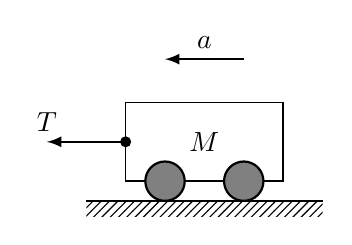
\begin{tikzpicture}[>=latex, thick]
  \begin{scope}[xshift=5cm,yshift=-1.5cm]
  \fill [pattern =north east lines](-1.5, 0) rectangle (1.5, -.2);
  \draw [thick](-1.5,0)--(1.5,0);
  \draw [semithick](-1,.25) rectangle (1,1.25);
  \draw [thick,->](-1,.75)--(-2,.75)node [above]{$T$};
  \fill (-1,.75) circle(2pt);
  \draw [thick,->](.5,1.8)--node [above]{$a$}(-.5,1.8);
  \node at (0,.75){$M$};
  \draw [fill=gray] (-.5, .25) circle (0.25);
  \draw [fill=gray] (.5, .25) circle (0.25);
  \end{scope}
\end{tikzpicture}
\end{document}